%El presente capítulo describe el modelo de negocios para el módulo de Registro de escuelas, el cual es utilizado dentro del desarrollo del {\bf \varProyecto}, el cual se conforma de los siguientes elementos:

El presente capítulo describe el modelo de negocios correspondiente al \saear , el cual se conforma de los siguientes elementos:

\begin{itemize}

    \item Modelo del ciclo de vida de una cuenta para su activación. Define la evolución de una cuenta desde que se encuentra inactiva, hasta que se activa mediante la verificación de correo electrónico.
    
    \item Modelo del ciclo de vida de una escuela durante su participación en el programa. Define la evolución de una escuela desde su solicitud de inscripción hasta que obtiene su acreditación en el programa.

    \item Modelo de información. En esta sección se presentan los atributos y relaciones de toda la información que contemplará el sistema en los módulos de Registro de escuelas, Información base para indicadores, Plan de acción, Seguimiento y acreditación e Indicadores.

    \item Reglas de negocio. Son las directivas destinadas a gobernar, guiar o influenciar el comportamiento de los procesos de negocio.
     %Son las directivas que expresan una política de negocio, es decir, describen, limitan o controlan un determinado aspecto del negocio.\\

\end{itemize}

%===============================================================================================
\section{Modelo del ciclo de vida de una cuenta para su activación} \label{subsec:cuenta:maquina} \hypertarget{subsec:cuenta:maquina}{}

Una cuenta puede pasar por una serie de etapas o ``estados'' para estar activa en el sistema, los cuales se asignan desde que se registra al \cdtRef{actor:usuarioEscuela}{Coordinador del programa} y culminan con la verificación de correo electrónico por parte del mismo. El ciclo de vida de una cuenta para estar activa, sus estados y transiciones se muestran en la figura \ref{fig:maquinaEstadosCuenta} y se describen a continuación.

  \begin{figure}[htbp!]
  \centering
      \fbox{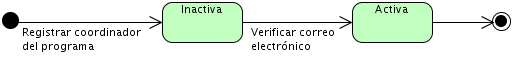
\includegraphics[width=\textwidth]{images/maquinasEstados/maquinaEstadosCuenta}}
      \caption{Modelo del ciclo de vida de una cuenta para su activación}
      \label{fig:maquinaEstadosCuenta}
  \end{figure}

\begin{description}

     \BRterm{estado:inactiva}{\bf Inactiva:} Éste estado ocurre una vez que se registra al \cdtRef{actor:usuarioEscuela}{Coordinador del programa} y que se envía por parte del sistema el correo de verificación de cuenta.

     \BRterm{estado:activa}{\bf Activa:} La cuenta pasa a éste estado cuando el \cdtRef{actor:usuarioEscuela}{Coordinador del programa} realiza la verificación de su correo electrónico.
     
\end{description}

%===============================================================================================
\section{Modelo del ciclo de vida de una escuela durante su participación en el programa} \label{subsec:escuela:maquina} \hypertarget{subsec:escuela:maquina}{}

Una escuela puede pasar por una serie de etapas o ``estados'' para estar inscrita, los cuales se asignan desde su solicitud de inscripción hasta su acreditación. El ciclo de vida que describe la participación de una escuela en el programa, sus estados y transiciones se muestran en la figura \ref{fig:maquinaEstadosEscuelas} y se describen a continuación.

  \begin{figure}[htbp!]
  \centering
      \fbox{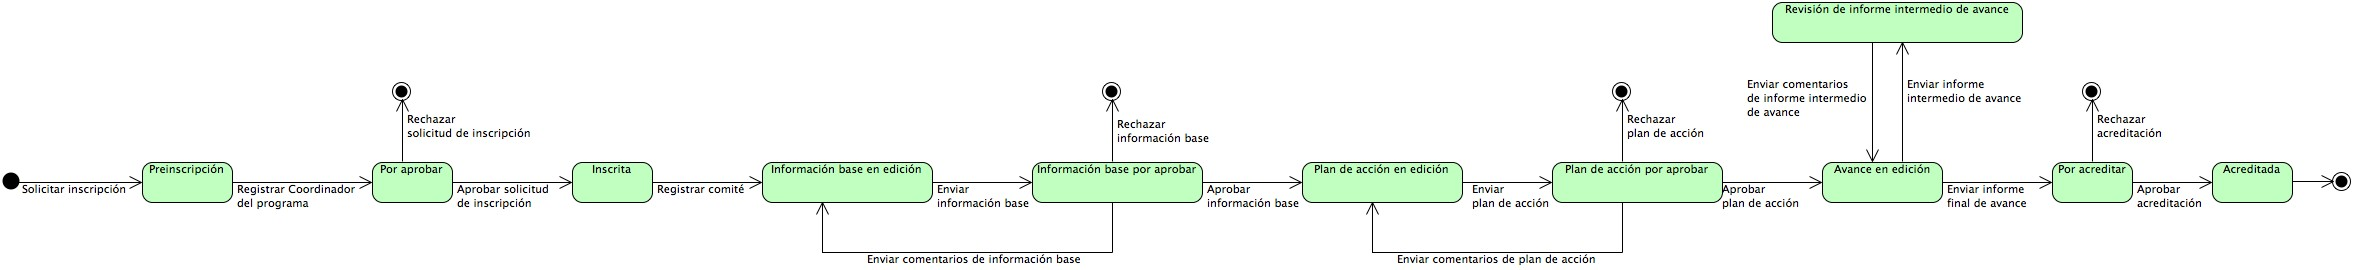
\includegraphics[width=\textwidth]{images/maquinasEstados/maquinaEstadosEscuela}}
      \caption{Modelo del ciclo de vida de una escuela durante su participación en el programa}
      \label{fig:maquinaEstadosEscuelas}
  \end{figure}

\begin{description}


     \BRterm{estado:preinscripcion}{\bf Preinscripción:} El director de la escuela es el encargado de solicitar la inscripción de su escuela en el programa, verificando la información de su escuela de acuerdo a lo registrado en el catálogo de la DGAIR (Dirección General de Acreditación, Inscripción y Revalidación). Una vez verificada la información, en este estado el director de la escuela debe registrarse como \cdtRef{actor:usuarioEscuela}{Coordinador del programa} y adjuntar los archivos correspondientes a su nombramiento como director y su carta compromiso para el programa.

      \BRterm{estado:aprobar}{\bf Por aprobar:} En este estado el \cdtRef{actor:usuarioSMAGEM}{Director del programa} en la SMAGEM puede visualizar la información de las escuelas que han solicitado su inscripción al programa. Cuando una escuela se encuentra en este estado significa que su información registrada, así como los archivos adjuntos deberán ser revisados para decidir si se aprueba o rechaza su solicitud de inscripción. En caso de que la información sea correcta se aprueba la solicitud de inscripción de la escuela, en caso contrario se rechaza.

%      \BRterm{estado:rechazada}{\bf Rechazada:} Cuando la escuela se encuentra en este estado, quiere decir que la información proporcionada por el director de la escuela es incorrecta, por lo que la información enviada en el estado de ``Preinscripción'' se elimina del sistema y se envía al \cdtRef{actor:usuarioEscuela}{Coordinador del programa} un correo electrónico de información errónea.

      \BRterm{estado:inscrita}{\bf Inscrita:} Este estado se presenta cuando se aprobó la solicitud de inscripción de la escuela a partir del estado ``Por aprobar'', y significa que la información proporcionada en el estado de  ``Preinscripción'' es correcta, por lo que el sistema envía al \cdtRef{actor:usuarioEscuela}{Coordinador del programa} un correo electrónico con su usuario y contraseña para ingresar en el sistema.

      \BRterm{estado:infoBaseEdicion}{\bf Información base en edición:} La escuela se encuentra en este estado cuando el \cdtRef{actor:usuarioEscuela}{Coordinador del programa} termina de registrar su comité escolar, o cuando el \cdtRef{actor:usuarioSMAGEM}{Director del programa} en la SMAGEM envía cometarios sobre la primera revisión de la información base para indicadores desde el estado ``Información base por aprobar''. En este estado el \cdtRef{actor:usuarioEscuela}{Coordinador del programa} puede relizar el registro o modificación de la información base para indicadores.

      \BRterm{estado:infoBaseAprobar}{\bf Información base por aprobar:} Este estado se presenta una vez que el \cdtRef{actor:usuarioEscuela}{Coordinador del programa} envía a la SMAGEM su información base para indicadores para ser revisada. En este estado el \cdtRef{actor:usuarioSMAGEM}{Director del programa} en la SMAGEM podrá aceptar la información base recibida, enviar comentarios de una primera revisión o rechazar dicha información en una segunda revisión.

      \BRterm{estado:planEdicion}{\bf Plan de acción en edición:} La escuela se encuentra en este estado cuando el \cdtRef{actor:usuarioSMAGEM}{Director del programa} en la SMAGEM aprueba la información base de la escuela desde el estado ``Información base por aprobar'', o cuando el \cdtRef{actor:usuarioSMAGEM}{Director del programa} en la SMAGEM envía cometarios sobre la primera revisión del plan de acción desde el estado ``Plan de acción por aprobar''. En este estado el \cdtRef{actor:usuarioEscuela}{Coordinador del programa} puede relizar el registro o modificación de su plan de acción.

      \BRterm{estado:planAprobar}{\bf Plan de acción por aprobar:} Este estado se presenta una vez que el \cdtRef{actor:usuarioEscuela}{Coordinador del programa} envía a la SMAGEM su plan de acción para ser revisado. En este estado el \cdtRef{actor:usuarioSMAGEM}{Director del programa} en la SMAGEM podrá aceptar el plan de acción recibido, enviar comentarios de una primera revisión o rechazar el plan de acción en una segunda revisión.

      \BRterm{estado:avanceEdicion}{\bf Avance en edición:} La escuela se encuentra en este estado cuando el \cdtRef{actor:usuarioSMAGEM}{Director del programa} en la SMAGEM aprueba el plan de acción de la escuela desde el estado ``Plan de acción por aprobar'', o cuando el \cdtRef{actor:usuarioSMAGEM}{Director del programa} en la SMAGEM envía cometarios sobre el informe intermedio de avance desde el estado ``Revisión de informe intermedio de avance''. En este estado el \cdtRef{actor:usuarioEscuela}{Coordinador del programa} puede relizar el registro o modificación de sus avances de plan de acción.

      \BRterm{estado:informeIntermedio}{\bf Revisión de informe intermedio de avance:} Este estado se presenta cuando el \cdtRef{actor:usuarioEscuela}{Coordinador del programa} envía a la SMAGEM su informe intermedio de avance para ser revisado. En este estado el \cdtRef{actor:usuarioSMAGEM}{Director del programa} en la SMAGEM podrá realizar la revisión de los informes intermedios de avance del plan de acción de las escuelas y enviar sus comentarios.
      
      \BRterm{estado:porAcreditar}{\bf Por acreditar:} La escuela se encuentra en este estado cuando el \cdtRef{actor:usuarioEscuela}{Coordinador del programa} envía su informe final de avance de plan de acción. En este estado el \cdtRef{actor:usuarioSMAGEM}{Director del programa} en la SMAGEM podrá revisar la información proporcionada por parte de las escuelas y aprobar o rechazar su acreditación.
 
      \BRterm{estado:acreditada}{\bf Acreditada:} Este estado se presenta cuando se aprueba la acreditación de la escuela dentro del programa por parte del \cdtRef{actor:usuarioSMAGEM}{Director del programa} en la SMAGEM. En este estado el \cdtRef{actor:usuarioEscuela}{Coordinador del programa} podrá visualizar el nivel de acreditación obtenido.

\end{description}
